% !Tex root = main.tex
% \chapter{Návrh softvérového diela}
% V tejto kapitole vysvetľujeme a popisujeme vstupné a vystúpné dáta a aj kód implementovaného programu. Vlastnosti vstupných dát, ich pôvod a iné veci, ktore spomíname sa nachádzajú v článku~\cite{10.1145/3307772.3328313}. Odkaz, pomocou ktorého je možné vstupné dáta získať sa tiež nachádza v článku~\cite{10.1145/3307772.3328313}.
% \section{Vstupné dáta}
% % \section{Vstupné dáta.}
% % \section{Trénovacie dáta.}
% % \section{Trénovacie dáta}
% % \section{Testovacie dáta}
% % \section{Testovacie dáta.}

% Dáta, z ktoré čerpáme pochádzajú z 2 adaptívnych nabíjacích sieti (anglická skratka je ACN), ktoré sa nachádzajú v Kalifornií. Nabíjacia sieť Caltechu je dostupná verejnosti, zatiaľ čo nabíjaciu sieť JPL môžu používať len zamestnanci.


% % Dáta z ACN-data majú tvar:

% \begin{figure}[H]
%     \begin{center}
%     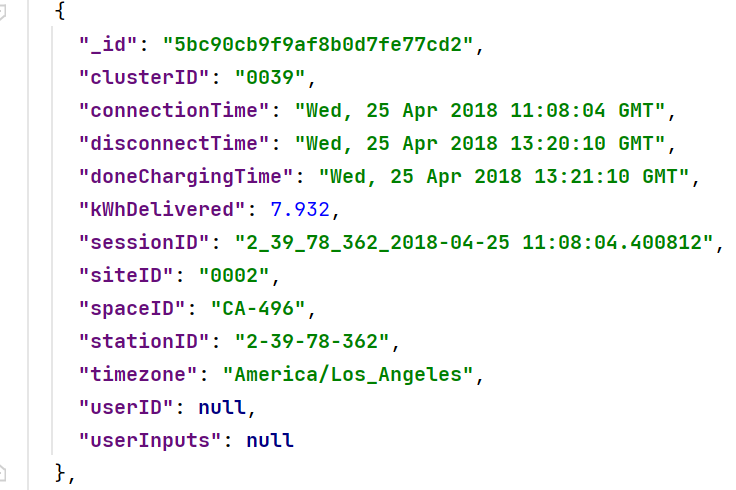
\includegraphics{images/acndata.png}
%     \caption{Dáta z Caltech adaptívnej nabíjacej siete.}
%     \end{center}
%     \label{imp:t:caltech}
% \end{figure}
% Kde pre nás najpodstatnejšie  premenné sú connectionTime, disconnectTime a kWHDelivered. Tieto premenné reprezentujeme pomocou trojice $(a(j), d(j), e(j))$.

% % al pouzit H
% % Dáta z pracoviska JPL majú tvar:
% \begin{figure}[H]
%     \begin{center}
%     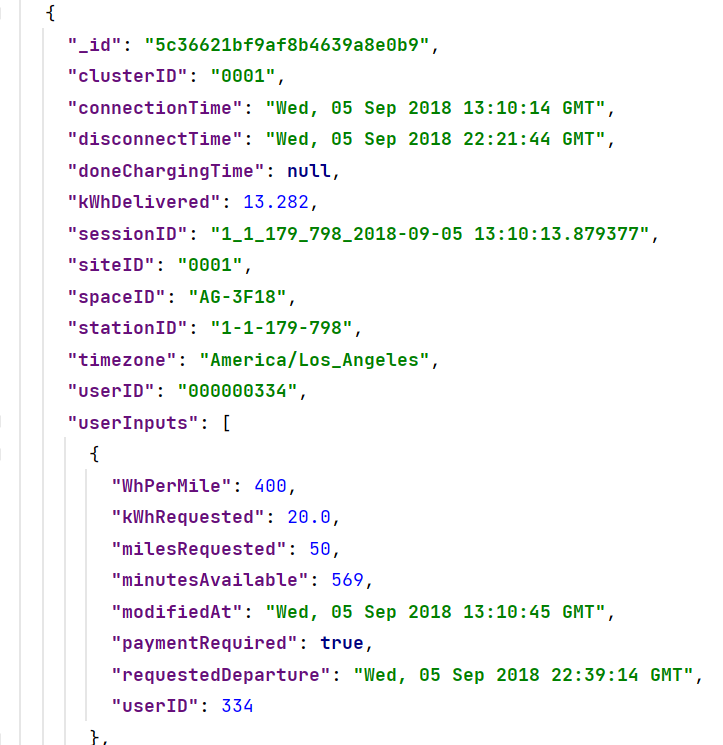
\includegraphics{images/jpldata.png}
%     \caption{Dáta z JPL adaptívnej nabíjacej siete.}
%     \end{center}
%     \label{imp:t:jpl}
% \end{figure}




